\chapter{Problem Formulation}
\label{chapter:problemformulation}

\textcolor{red}{\textbf{This part is incomplete, I am now writing the strategy part}}\newline
We formulate the problem in following way

\section{Runtime Exceptions}
\label{subsec:excep}

\begin{figure}[htb]
\centering
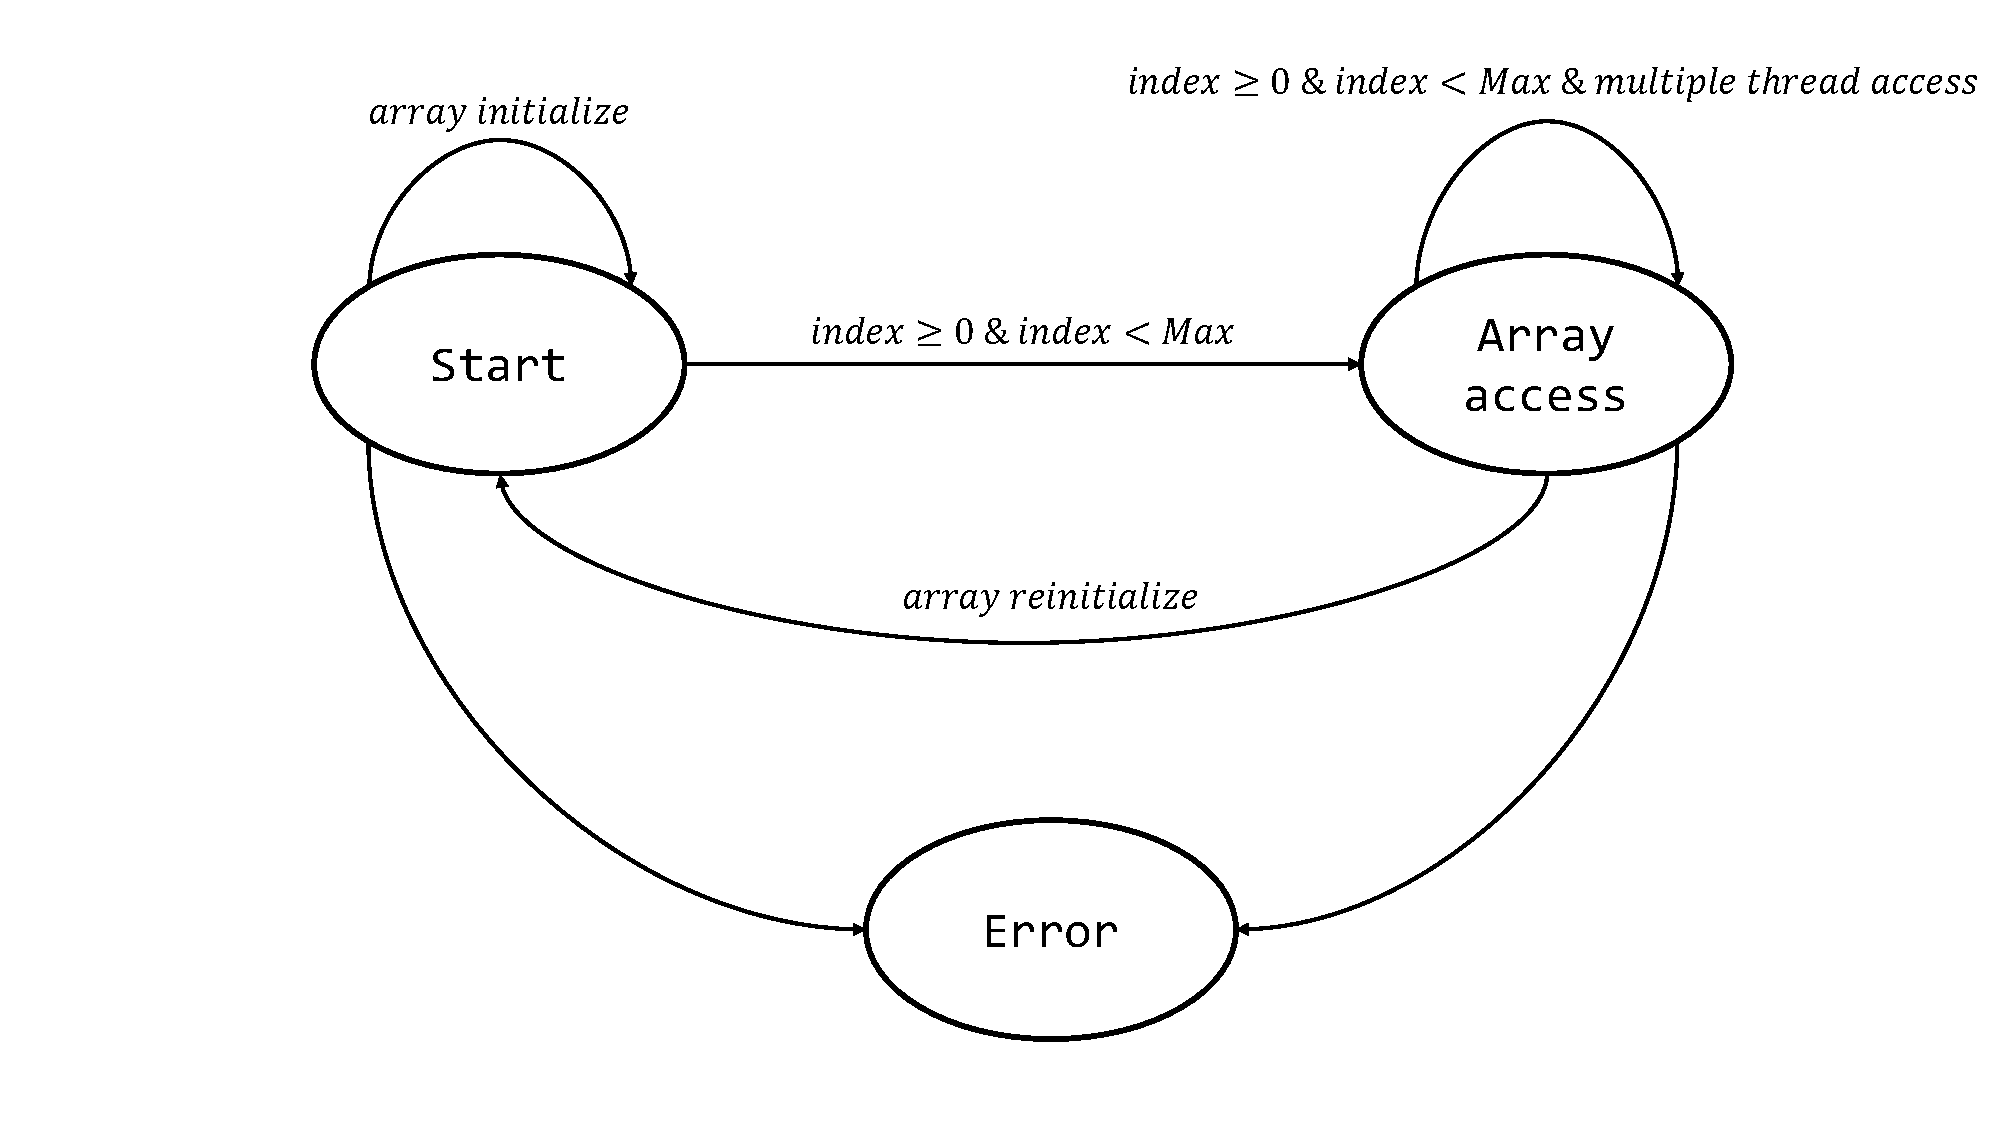
\includegraphics[width=0.65\textwidth]{images/ArrayIndex.pdf}
\caption{array index out of bound formulated as FSM }
\label{fig:array}
\end{figure}


We can visualize all runtime exceptions as finite state machine (FSM). When a
program violates such sequence, it throws runtime exception.
In Figure~\ref{fig:array}, array index out of bound (java.lang.
ArrayIndexOutOfBoundException) exception is described as a FSM.
Here, a program will be in safe bound as long as the $array\_index \geq 0$ or
$array\_index \leq max\_array\_size - 1$

